% ========================================
%	Header einbinden
% ========================================

\documentclass[bibtotoc,titlepage]{scrartcl}

% Deutsche Spracheinstellungen
\usepackage[ngerman,german]{babel, varioref}
\usepackage[T1]{fontenc}
\usepackage[utf8]{inputenc}

%\usepackage{marvosym}

\usepackage{amsfonts}
\usepackage{amssymb}
\usepackage{amsmath}
\usepackage{amscd}
\usepackage{amstext}
\usepackage{float}
\usepackage{caption}
\usepackage{wrapfig}
\usepackage{setspace}
\usepackage{threeparttable}
\usepackage{footnote}

\usepackage{caption}
\usepackage{subcaption}

\newfloat{formel}{htbp}{for}
\floatname{formel}{Formel}


\usepackage{longtable}

%\usepackage{bibgerm}

\usepackage{footnpag}

\usepackage{ifthen}                 %%% package for conditionals in TeX
\usepackage{siunitx}
%Fr textumflossene Bilder und Tablellen
%\usepackage{floatflt} - veraltet

%Fr Testzwecke aktivieren, zeigt labels und refs im Text an.
%\usepackage{showkeys}

% Abstand zwischen zwei Abs�zen nach DIN (1,5 Zeilen)
% \setlength{\parskip}{1.5ex plus0.5ex minus0.5ex}

% Einrckung am Anfang eines neuen Absatzes nach DIN (keine)
%\setlength{\parindent}{0pt}

% R�der definieren
% \setlength{\oddsidemargin}{0.3cm}
% \setlength{\textwidth}{15.6cm}

% bessere Bildunterschriften
%\usepackage[center]{caption2}


% Probleml�ungen beim Umgang mit Gleitumgebungen
\usepackage{float}

% Nummeriert bis zur Strukturstufe 3 (also <section>, <subsection> und <subsubsection>)
%\setcounter{secnumdepth}{3}

% Fhrt das Inhaltsverzeichnis bis zur Strukturstufe 3
%\setcounter{tocdepth}{3}

\usepackage{exscale}

\newenvironment{dsm} {\begin{displaymath}} {\end{displaymath}}
\newenvironment{vars} {\begin{center}\scriptsize} {\normalsize \end{center}}


\newcommand {\en} {\varepsilon_0}               % Epsilon-Null aus der Elektrodynamik
\newcommand {\lap} {\; \mathbf{\Delta}}         % Laplace-Operator
\newcommand {\R} { \mathbb{R} }                 % Menge der reellen Zahlen
\newcommand {\e} { \ \mathbf{e} }               % Eulersche Zahl
\renewcommand {\i} { \mathbf{i} }               % komplexe Zahl i
\newcommand {\N} { \mathbb{N} }                 % Menge der nat. Zahlen
\newcommand {\C} { \mathbb{C} }                 % Menge der kompl. Zahlen
\newcommand {\Z} { \mathbb{Z} }                 % Menge der kompl. Zahlen
\newcommand {\limi}[1]{\lim_{#1 \rightarrow \infty}} % Limes unendlich
\newcommand {\sumi}[1]{\sum_{#1=0}^\infty}
\newcommand {\rot} {\; \mathrm{rot} \,}         % Rotation
\newcommand {\grad} {\; \mathrm{grad} \,}       % Gradient
\newcommand {\dive} {\; \mathrm{div} \,}        % Divergenz
\newcommand {\dx} {\; \mathrm{d} }              % Differential d
\newcommand {\cotanh} {\; \mathrm{cotanh} \,}   %Cotangenshyperbolicus
\newcommand {\asinh} {\; \mathrm{areasinh} \,}  %Area-Sinus-Hyp.
\newcommand {\acosh} {\; \mathrm{areacosh} \,}  %Area-Cosinus-H.
\newcommand {\atanh} {\; \mathrm{areatanh} \,}  %Area Tangens-H.
\newcommand {\acoth} {\; \mathrm{areacoth} \,}  % Area-cotangens
\newcommand {\Sp} {\; \mathrm{Sp} \,}
\newcommand {\mbe} {\stackrel{\text{!}}{=}}     %Must Be Equal
\newcommand{\qed} { \hfill $\square$\\}
\renewcommand{\i} {\imath}
\def\captionsngerman{\def\figurename{\textbf{Abb.}}}

%%%%%%%%%%%%%%%%%%%%%%%%%%%%%%%%%%%%%%%%%%%%%%%%%%%%%%%%%%%%%%%%%%%%%%%%%%%%
% SWITCH FOR PDFLATEX or LATEX
%%%%%%%%%%%%%%%%%%%%%%%%%%%%%%%%%%%%%%%%%%%%%%%%%%%%%%%%%%%%%%%%%%%%%%%%%%%%
%%%
\ifx\pdfoutput\undefined %%%%%%%%%%%%%%%%%%%%%%%%%%%%%%%%%%%%%%%%% LATEX %%%
%%%
\usepackage[dvips]{graphicx}       %%% graphics for dvips
\DeclareGraphicsExtensions{.eps,.ps}   %%% standard extension for included graphics
\usepackage[ps2pdf]{thumbpdf}      %%% thumbnails for ps2pdf
\usepackage[ps2pdf,                %%% hyper-references for ps2pdf
bookmarks=true,%                   %%% generate bookmarks ...
bookmarksnumbered=true,%           %%% ... with numbers
hypertexnames=false,%              %%% needed for correct links to figures !!!
breaklinks=true,%                  %%% breaks lines, but links are very small
linkbordercolor={0 0 1},%          %%% blue frames around links
pdfborder={0 0 112.0}]{hyperref}%  %%% border-width of frames
%                                      will be multiplied with 0.009 by ps2pdf
%
%\hypersetup{ pdfauthor   = {Hannes Franke; Julius Tilly},
%pdftitle    = {x}, pdfsubject  = {Protokoll FP}, pdfkeywords = {V301, Innenwiderstand, Leistungsanpassung},
%pdfcreator  = {LaTeX with hyperref package}, pdfproducer = {dvips
%+ ps2pdf} }
%%%
\else %%%%%%%%%%%%%%%%%%%%%%%%%%%%%%%%%%%%%%%%%%%%%%%%%%%%%%%%%% PDFLATEX %%%
%%%
\usepackage[pdftex]{graphicx}      %%% graphics for pdfLaTeX
\DeclareGraphicsExtensions{.pdf}   %%% standard extension for included graphics
\usepackage[pdftex]{thumbpdf}      %%% thumbnails for pdflatex
\usepackage[pdftex,                %%% hyper-references for pdflatex
bookmarks=true,%                   %%% generate bookmarks ...
bookmarksnumbered=true,%           %%% ... with numbers
hypertexnames=false,%              %%% needed for correct links to figures !!!
breaklinks=true,%                  %%% break links if exceeding a single line
linkbordercolor={0 0 1},
linktocpage]{hyperref} %%% blue frames around links
%                                  %%% pdfborder={0 0 1} is the default
% \hypersetup{
% pdftitle    = {V301 Innenwiderstand und Leistungsanpassung}, 
% pdfsubject  = {Protokoll AP}, 
% pdfkeywords = {V301, Innenwiderstand, Leistungsanpassung},
% pdfsubject  = {Protokoll AP},
% pdfkeywords = {V301, Innenwiderstand, Leistungsanpassung}}
%                                  %%% pdfcreator, pdfproducer,
%                                      and CreationDate are automatically set
%                                      by pdflatex !!!
\pdfadjustspacing=1                %%% force LaTeX-like character spacing
\usepackage{epstopdf}
%
\fi %%%%%%%%%%%%%%%%%%%%%%%%%%%%%%%%%%%%%%%%%%%%%%%%%%% END OF CONDITION %%%
%%%%%%%%%%%%%%%%%%%%%%%%%%%%%%%%%%%%%%%%%%%%%%%%%%%%%%%%%%%%%%%%%%%%%%%%%%%%
% seitliche Tabellen und Abbildungen
%\usepackage{rotating}
\usepackage{ae}
\usepackage{
  array,
  booktabs,
  dcolumn
}
\makeatletter 
  \renewenvironment{figure}[1][] {% 
    \ifthenelse{\equal{#1}{}}{% 
      \@float{figure} 
    }{% 
      \@float{figure}[#1]% 
    }% 
    \centering 
  }{% 
    \end@float 
  } 
  \makeatother 


  \makeatletter 
  \renewenvironment{table}[1][] {% 
    \ifthenelse{\equal{#1}{}}{% 
      \@float{table} 
    }{% 
      \@float{table}[#1]% 
    }% 
    \centering 
  }{% 
    \end@float 
  } 
  \makeatother 
%\usepackage{listings}
%\lstloadlanguages{[Visual]Basic}
%\allowdisplaybreaks[1]
%\usepackage{hycap}
%\usepackage{fancyunits}

% ========================================
%	Angaben für das Titelblatt
% ========================================

\title{Debye-Scherrer Aufnahmen\\				% Titel des Versuchs 
\large TU Dortmund, Fakultät Physik\\ 
\normalsize Fortgeschrittenen-Praktikum}

\author{Jan Adam\\			% Name Praktikumspartner A
{\small \href{jan.adam@tu-dortmund.de}{jan.adam@tu-dortmund.de}}	% Erzeugt interaktiven einen Link
\and						% um einen weiteren Author hinzuzfügen
Dimitrios Skodras\\					% Name Praktikumspartner B
{\small \href{dimitrios.skodras@tu-dortmund.de}{dimitrios.skodras@tu-dortmund.de}}		% Erzeugt interaktiven einen Link
}
\date{27. Mai 2015}				% Das Datum der Versuchsdurchführung

% ========================================
%	Das Dokument beginnt
% ========================================

\begin{document}

% ========================================
%	Titelblatt erzeugen
% ========================================

\maketitle					% Jetzt wird die Titelseite erzeugt
\thispagestyle{empty} 				% Weder Kopfzeile noch Fußzeile

% ========================================
%	Der Vorspann
% ========================================

%\newpage					% Wenn Verzeichnisse auf einer neuen Seite beginnen sollen
%\pagestyle{empty}				% Weder Kopf- noch Fußzeile für Verzeichnisse

\tableofcontents

%\newpage					% eine neue Seite
%\thispagestyle{empty}				% Weder Kopf- noch Fußzeile für Verzeichnisse
%\listoffigures					% Abbildungsverzeichnis

%\newpage					% eine neue Seite
%\thispagestyle{empty}				% Weder Kopf- noch Fußzeile für Verzeichnisse
%\listoftables					% Tabellenverzeichnis
\newpage					% eine neue Seite


% ========================================
%	Kapitel
% ========================================

%\section{Einleitung}				% Bei Bedarf

\section{Theorie}\label{sec:theorie}
Viele makroskopische Eigenschaften von Materie können auf den Aufbau ihrer Grundbausteine, dh. Atome und Moleküle zurückgeführt werden. Bei Feststoffen liegen diese in kristalliner Form vor und bilden regelmäßig auftretende Strukturen, sog. Gitter aus. Durch die Untersuchung dieser Gitter können wichtige tensorielle und vektorielle makroskopische Eigenschaften, wie zum Beispiel Elastizität und Permeabilität bestimmt werden. Um die Gitterabstände auflösen zu können, die im $\mathring{A}$ngströmbereich liegen, ist die Wellenlänge des sichtbaren Lichtes zu groß. Röntgenstrahlen haben jedoch das benötigte Auflösungsvermögen.

\subsection{Über die Struktur der Materie}
Wie in \ref{sec:theorie} erwähnt, liegen die Atome von Festkörpern in Gitterstruktur vor. Diese können durch einen Translationsvektor
\begin{align}
	\vec{t} = n_1\vec{a} +n_2\vec{b} + n_3\vec{c}
\end{align}
beschrieben werden, der ausgehen von einem Startpunkt auf alle anderen Gitterpunkte zeigt, wenn man für die $n_i$ ganze Zahlen einsetzt. An den Gitterpunkten können entweder einzelne oder mehrere Atome sitzen. In letzterem Fall nennt man diese Ansammlung Basis. 

Da es für die $n_i$ keine Begrenzung gibt, existieren unendlich viele verschiedene Gitter. Hinsichtlich ihrer Symmetrieeigenschaften können sie jedoch im dreidimensionalen in 14 Gitterstrukturen zusammengefasst werden, den sog. Bravais-Gittern. Diese sind in 7 Gittersysteme unterteilt: triklin, monoklin, (ortho-)rhombisch, tetragonal, rhomboedrisch, hexagonal und kubisch. Alle Systeme und ihre Eigenschaften sind in Abbildung \ref{pic:bravais} aufgelistet.
\begin{figure}[htbp]
	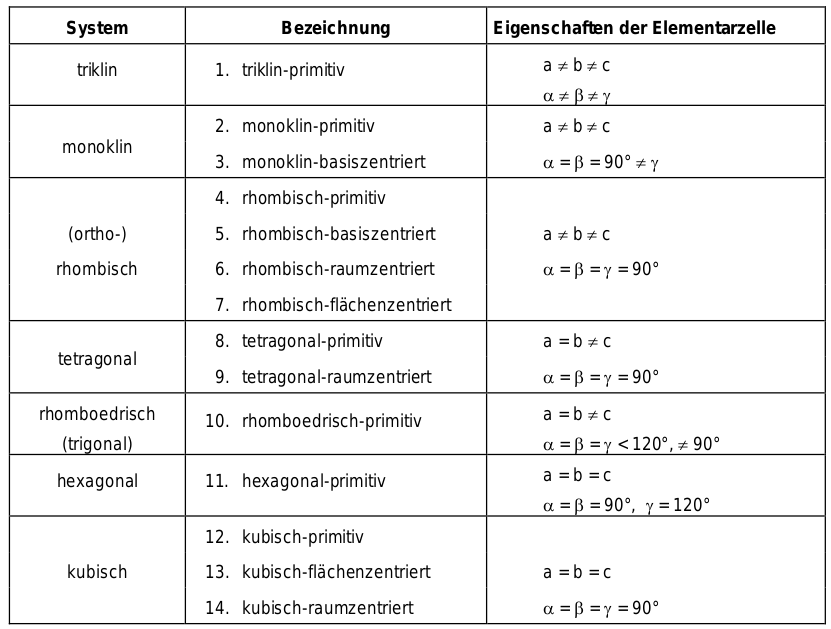
\includegraphics[width=0.9\textwidth]{../pics/bravais.png}
	\caption{Auflistung der 14 Bravaisgitter im dreidimensionalen Raum.}
	\label{pic:bravais}
\end{figure}
Besonderes Interesse  kommt dabei der sog. Elementarzelle zu. Dies ist die kleinste Einheit, die eine Kristallstruktur vollkommen festlegt. Beispielsweise kann man dazu das von den Vektoren a , b und c aufgespannte Parallelepiped benutzen. Liegen nur auf den Eckpunkten Atome, enthält die Zelle also im Ganzen nur ein einzelnes Atom, so nennt man sie primitiven Elementarzelle. 
Nicht jede Kristallstruktur lässt sich jedoch durch Vervielfachung einer primitiven Elementarzelle aufbauen. Die in diesem Versuch untersuchten Stoffe haben eine kubische Grundstruktur, daher wird nur dieses System im Folgenden detaillierter beschrieben. In Abbildung \ref{pic:gitterTyp} sind die zwei möglichen Abwandlungen des kubischen Bravais-Gitters dargestellt.
\begin{figure}[htbp]
	\centering
	\begin{subfigure}[b]{0.3\textwidth}
		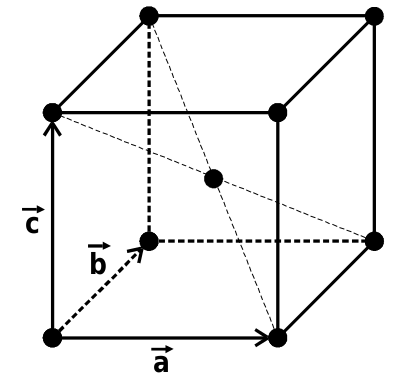
\includegraphics[width=\textwidth]{../pics/bcc.png}
		\caption{bcc-Gitter}
		\label{pic:bcc}
	\end{subfigure}
	~ %add desired spacing between images, e. g. ~, \quad, \qquad, \hfill etc.
	%(or a blank line to force the subfigure onto a new line)
	\begin{subfigure}[b]{0.3\textwidth}
		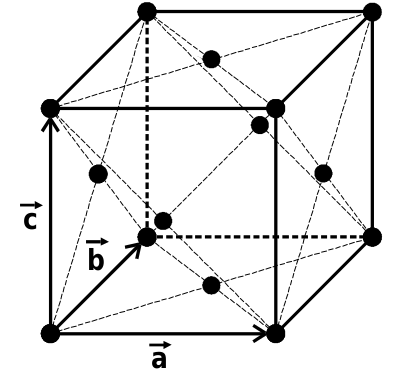
\includegraphics[width=\textwidth]{../pics/fcc.png}
		\caption{fcc-Gitter}
		\label{pic:fcc}
	\end{subfigure}
	\caption{Verschiedene}
	\label{pic:gitterTyp}
\end{figure}
Das kubisch-raumzentrierte \ref{pic:bcc} enthält zusätzlich zu den Eckpunkten noch ein weiteres Atom im Zentrum. Damit is es keine primitive Einheitszelle mehr, da die Zelle insgesamt 2 Atome enthält. Bei der kubisch-flächenzentrierten \ref{pic:fcc} Zelle sitzt dagegen auf jeder Flächenmitte ein weiteres Atom, wodurch die Einheitszelle sogar 4 Atome enthält.

Beschrieben werden diese verschiedenen Zelltypen durch die Position der Atome in der Basiszelle. Im Falle der primitiven Einheitszellen wäre dies lediglich ein Atom: $(0,0,0)$, im bcc Gitter zwei Atome: $(0,0,0)$ und $(\nicefrac{1}{2},\nicefrac{1}{2},\nicefrac{1}{2})$ und im fcc Gitter vier Atome: $(0,0,0)$, $(0,\nicefrac{1}{2},\nicefrac{1}{2})$, $(\nicefrac{1}{2},0,\nicefrac{1}{2})$ und $(\nicefrac{1}{2},\nicefrac{1}{2},0)$.

\subsection{Netzebenen}
Eine weitere wichtige Eigenschaft von Kristallen ist die Orientierung ihrer Netzebenen und deren Abstände.
Unter einer Netzebene im Kristall versteht man eine Ebene, in der Schwerpunkte von Atomen liegen. Die Gesamtheit aller Netzebenen, die zu einer vorgegebenen parallel liegen und daher äquidistant sind, bezeichnet man als Netzebenenschar. Ihre Orientierung wird durch die sog. Millerschen Indizes beschrieben. Diese sind ein Zahlentripel (hkl) aus natürlichen Zahlen und werden wie folgt bestimmt:
\begin{figure}[htbp]
	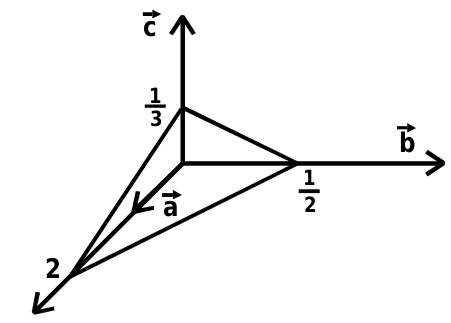
\includegraphics[width=0.3\textwidth]{../pics/miller.png}
	\caption{Bedeutung der Millerschen Indizes anhand eines Beispiels. Eingezeichnet sind eine Netzebene und der Koordinatenursprung mit seinen Achsen.}
	\label{pic:miller}
\end{figure}
In Abbildung \ref{pic:miller} schneidet eine Netzebene die Koordinatenachsen bei $2a$, $\nicefrac{1}{2}$ b und $\nicefrac{1}{3}$ c. Von diesen Zahlen nimmt man nun die Kehrwerte und multipliziert diese mit dem kleinsten gemeinsamen Vielfachen, damit man ganze Zahlen erhält. Die Millerschen Indizes wären in diesem Fall also $(hkl) = (146)$. Negative Zahlen werden mit einem Strich $-4 \rightarrow \bar{4}$ gekennzeichnet und wenn eine Achse garnicht (im unendlichen) geschnitten wird, so ist der Indize $\nicefrac{1}{\infty}=0$.

Für das kubische Kristallsystem lässt sich so auch der Netzebenabstand sehr einfach durch die Millerschen Indizes und der Gitterkonstanten a ausdrücken:
\begin{align}
d = \frac{a}{\sqrt{h^2 + k^2 + l^2}}
\label{eq:gapMiller}
\end{align}

\subsection{Röntgenreflexion und Interferenz}
Wird ein Kristall Röntgenstrahlung ausgesetzt, so werden die Elektronenhüllen der Atome an den Gitterplätzen zu Schwingungen angeregt und emittieren ihrerseits die Strahlung wieder. Da die Gitterplätze räumlich streng periodisch angeordnet sind, kann dadurch Interferenz auftreten. In Abbildung +++++ ist der geometrische Zusammenhang zum Gangunterschied $\Delta s$ dargestellt. Wenn dieser ein ganzzahliges Vielfaches der Wellenlänge $\lambda$ ist, so interferieren die Wellen konstruktiv und ein Röntgenreflex kann unter dem Winkel $\Theta$ festgestellt werden. Zusammen mit dem Netzebenabstand $d$ lautet die Interferenzbedingung für konstruktive Interferenz an parallelen Netzebenen:
\begin{align}
 \lambda = 2 d \sin(\theta)
 \label{eq:bragg}
\end{align}
Dies ist die sog. Braggsche Bedingung.

\section{Durchführung}
In diesem Versuch sollen die Elementarzellen eines Kristalls durch Röntgenreflexe untersucht werden. Dazu wird ein Kristall fein zerstäubt und auf ein Probenstäbchen wie in Abbildung \ref{pic:aufbau} aufgetragen.
\begin{figure}[htbp]
	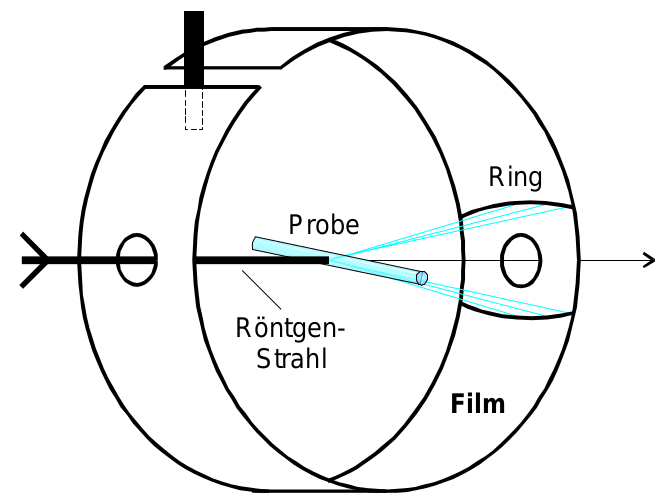
\includegraphics[width=0.6\textwidth]{../pics/aufbau.png}
	\caption{Im Versuch verwendeter Aufbau. Zusehen ist das zentrale Probenstäbchen, welches von den Röntgenstrahlen getroffen wird und Interferenzringe auf den Filmstreifen wirft.}
	\label{pic:aufbau}
\end{figure}
Die Probe wird deshalb zerstäubt, da Interferenz nur beim richtigen Winkel auftritt und ein Einkristall a priori nicht korrekt ausgerichtet werden kann. Durch das zerstäuben werden viele kleine Mikrokristalle erzeugt und zufällig ausgerichtet, so dass immer eine ausreichend große Anzahl die richtige Ausrichtung aufweist. Um die Trefferquote zu erhöhen, wird zudem das Probenstäbchen durch einen Motor langsam gedreht. 

Die Probe befindet sich in einer komplett verdunkelten Filmdose, die nur zwei Öffungen für den ein- und austretenden Strahl hat. In der Mantelfläche ist ein Fotofilm angebracht, der sich durch die reflektierte Röntgenstrahlung schwarz färbt. Mit diesem Filmstreifen können im Anschluss die Reflektionswinkel bestimmt werden.

Jeder Mikrokristall erzeugt einen eigenen Röntgenreflex, die zwar alle unter dem gleichen Winkel, jedoch in eine andere Richtung ausfallen. Durch die zufällige Verteilung der Mikrokristalle ist als Summe ein kreisförmiger Reflex auf dem Fotofilm zu sehen.


\section{Auswertung}
\subsection{Bestimmung der Gitterkonstanten}

Mit einem Lineal werden entsprechend Abbildung \ref{pic:debyefilm} die Abstände $r_i$ der Debye-Sherrer-Reflexringe zum Austrittsloch gemessen. Der 
Beugungswinkel kann nun mit $\theta_i = r_i/R$ errechnet werden, wobei $R=57,4$ mm der Kameraradius ist. 
\begin{figure}[H]
 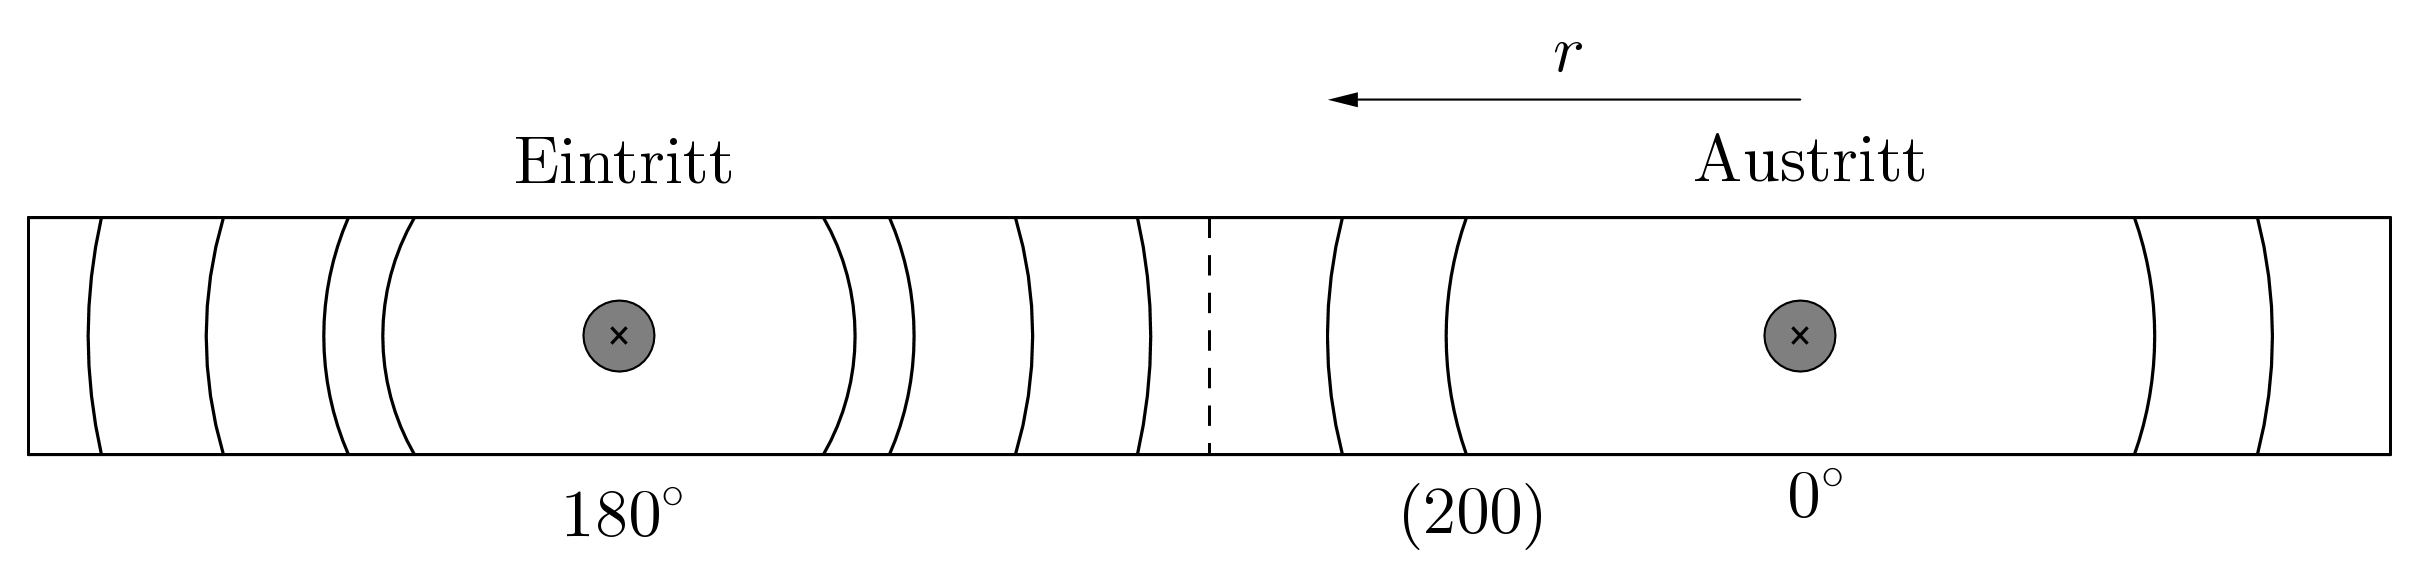
\includegraphics[width=\textwidth]{../pics/debyestreifen.jpg}
 \caption{Debye Filmaufnahme}
 \label{pic:debyefilm}
\end{figure}
\noindent Ausgehend davon, dass der Reflex beim niederwertigsten
Winkel $\theta_0$ an der (200)-Ebene gestreut wird, seien die experimentellen Strukturfaktoren $s^\text{exp}_i$ gegeben durch
\begin{align}
 s^\text{exp}_i = 4\frac{\sin^2(\theta_i)}{\sin^2(\theta_0)},
 \label{eq:structExp}
\end{align}
hervorgehend aus der Bragg-Gleichung \eqref{eq:bragg} und \eqref{eq:gapMiller}. Nun werden die entsprechenden $(h_ik_il_i)$-Tripel sinnvoll geraten und als 
$s^\text{theo}_i$ mit
\begin{align}
 s^\text{theo}_i = h_i^2 + k_i^2 + l_i^2
 \label{eq:structTheo}
\end{align}
bezeichnet, wobei die Millerindizes (MI) zum $i$-ten Reflex gehören. Damit kann man bereits den Gitterparameter $a$ berechnen als
\begin{align}
 a_i = \lambda\frac{\sqrt{s^\text{theo}_i}}{2\sin(\theta)}.
 \label{eq:gitterparameter}
\end{align}
mit $\lambda=154$ nm als Wellenlänge der Röntgenstrahlen. Die bisher angesprochenen Größen sind in den Tabellen \ref{tab:messreihe1} und \ref{tab:messreihe2} zu finden.

\begin{table}[H]
 \begin{tabular}{cccccc}
$r$ in mm&	$\theta$ in $\pi$& $s^\text{exp}$& $s^\text{theo}$ & MI &$a$ in $\mathring{A}$\\
 \hline
32.0&	0.28&	4.00&	4&	200&	5.6\\
44.0&	0.38&	7.39&	8&	220&	5.83\\
53.0&	0.46&	10.48&	10&	310&	5.47\\
65.0&	0.57&	15.20&	14&	321&	5.38\\
81.0&	0.71&	22.22&	22&	332&	5.58 \\
  
 \end{tabular}
 \caption{Messwerte zur ersten Probe}
 \label{tab:messreihe1}

\end{table}

\begin{table}[H]
 \begin{tabular}{cccccc}
$r$ in mm&	$\theta$ in $\pi$& $s^\text{exp}$& $s^\text{theo}$ & MI &$a$ in $\mathring{A}$\\
\hline
31.0&	0.27&	4.00&	4&	200&	5.78\\
38.0&	0.33&	5.94&	6&	211&	5.81\\
44.0&	0.38&	7.86&	8&	220&	5.83\\
51.0&	0.44&	10.38&	10&	310&	5.67\\
65.0&	0.57&	16.17&	16&	400&	5.75\\
69.0&	0.60&	17.98&	18&	330&	5.78\\
74.0&	0.64&	20.29&	20&	420&	5.74\\
102.33&	0.89&	34.02&	34&	530&	5.78\\
106.33&	0.93&	35.91&	36&	600&	5.79\\
115.33&	1.00&	40.03&	40&	620&	5.78\\
119.33&	1.04&	41.78&	42&	541&	5.79\\
124.33&	1.08&	43.86&	44&	622&	5.79\\
134.33&	1.17&	47.66&	48&	444&	5.80\\
146.33&	1.27&	51.42&	51&	551&	5.76\\
  
 \end{tabular}
 \caption{Messwerte zur zweiten Probe}
 \label{tab:messreihe2}

\end{table}

\subsection{Korrektur zum Gitterparameter und Bestimmung der Proben}
Bei der Versuchsdurchführung treten zwei wesentliche, systematische Fehler auf. Zum einen ist eine Abhängigkeit des Gitterparameters vom Beugungswinkel,
was im Wesentlichen der Absorbtion der Röntgenstrahlen geschuldet ist. Und zum anderen fallen Probenachse und Filmzylinderachse nicht perfekt zusammen.
Es zeigt sich, dass bei der Apparatur der Fehler $\Delta a$ näherungsweise von der Summe beider Fehler und linear von $\cos^2(\theta)$ abhängt. Mittels
linearer Regression wird $a$ bei $\theta = 90^\circ$, also $\cos^2(\theta)=0$, als bester Wert angenommen (vgl. Abb. \ref{pic:fita1}, \ref{pic:fita2}). 

\begin{align}
 a_1 &= (519 \pm 52)\, \text{pm} \\
 \nonumber
 a_2 &= (578 \pm 2)\, \text{pm} 
 \label{eq:latticeResults}
\end{align}

\noindent




\section{Diskussion}
Das Debye-Scherrer Verfahren zur Bestimmung von Gitterparametern von kristallinen Stoffen ist sehr intuitiv und führt zu vernünftigen Resultaten, sodass
zur Probenbestimmung einige Kandidaten infrage kommen. Bei der Durchführung ist bekannt, dass ein Material ein Salz und das andere ein Metall ist. 

\noindent Anhand der Millerindizes für die erste Probe (vgl. Tabelle \ref{tab:messreihe1}) ergibt sich eine vermeintliche bcc-Struktur ($h+k+l$ ist gerade), 
die ähnlichzur NaCl-Struktur ist. Materialien mit einem Gitterparameter von $a_1 = 519 \pm 52$, die eine solche aufweisen, sind in Tabelle \ref{tab:matProb1} 
aufgeführt.

\begin{table}[H]
 \begin{tabular}{cc}
Material &$a$ in pm\\
\hline
MgS& 520\\
BaO & 554\\
SrO & 516\\
LiBr & 550\\
KF & 534
  
 \end{tabular}
 \caption{Kandidaten für die erste Probe mit NaCl-Struktur}
 \label{tab:matProb1}

\end{table}
\noindent Magnesiumsulfid hat jedoch einen nahezu perfekten Gitterparameter, jedoch ist die typische Farbe (rötlich) nicht mit der Probenfarbe gleich (weiß). 
Bariumoxid und Lithiumbromid sind zwar im Bereich des Messfehlers, aber eher im äußeren Teil. Daher handelt es sich vermutlich um Strontiumoxid oder
Kaliumflourid.

\noindent
Die Millerindizes der zweiten Probe (vgl. Tabelle \ref{tab:messreihe2}) sprechen für eine fcc-Struktur ($hkl$ alle gerade oder ungerade).
Für die fcc-Struktur, die vermutlich ein Metall aufweist, sind die Elemente des Periodensystems verglichen worden und die wahrscheinlichsten sind in 
Tabelle \ref{tab:matProb2} aufgeführt.

\begin{table}[H]
 \begin{tabular}{cc}
Material &$a$ in pm\\
\hline
Yb& 548\\
Sr & 608\\
Ge & 565\\
  
 \end{tabular}
 \caption{Kandidaten für die zweite Probe mit fcc-Struktur}
 \label{tab:matProb2}

\end{table}
\noindent Dass keines der genannten Stoffe im Fehlerbereich von $a_2$ liegt, sind zwei Ursachen denkbar. Zum einen kann es sich um einen Stoff halten, der nicht
rein aus einem Metall des Periodensystems besteht oder die fehlerhafte Abmessung der Debye-Scherrer-Ringe, die mit einem Geodreieck durchgeführt worden ist
sorgt für einschlägige Unterschiede für den Gitterparameter. Da es Unmengen an Legierungen gibt und verhältnismäßig wenig Literaturwerte über deren
Gitterkonstanten, ist darauf verzichtet worden, Kandidaten in diesem Feld zu suchen. Es ist zusätzlich möglich, dass auf den Fotostreifen, speziell
der zweiten Probe, Reflexe fehlinterpretiert mitaufgenommen oder nicht mitaufgenommen worden sind, was auf den geringen Konstrast zurückgeführt werden kann.

\begin{figure}[n]
 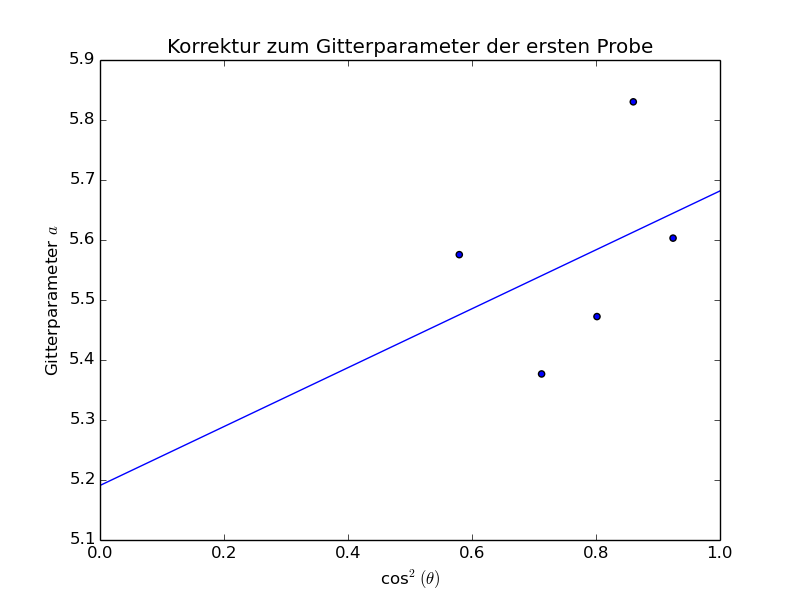
\includegraphics[width=0.7\textwidth]{../auswertung/a1.png}
 \caption{Korrigierter Wert für $a_1$ der Messreihe 1 bei $\cos(\theta)=0$}
 \label{pic:fita1}
\end{figure}

\begin{figure}[hb]
 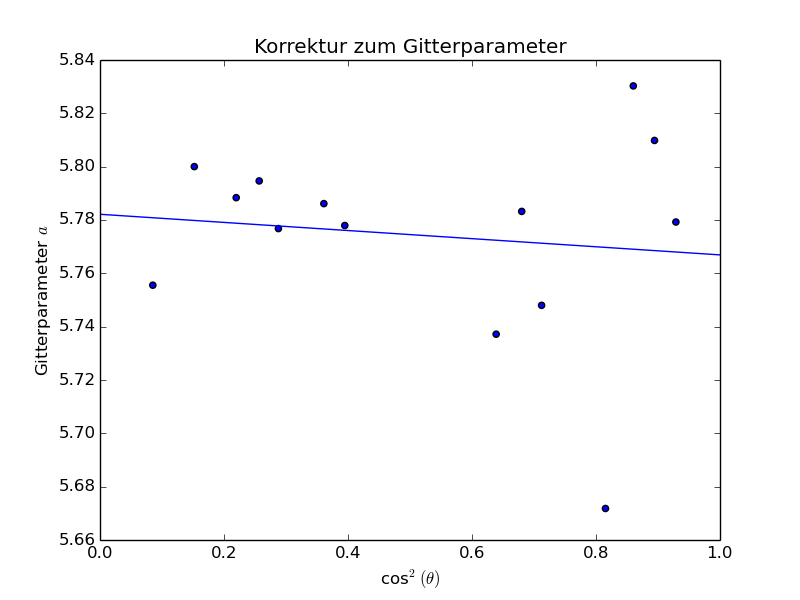
\includegraphics[width=0.7\textwidth]{../auswertung/a2.png}
 \caption{Korrigierter Wert für $a_2$ der Messreihe 2 bei $\cos(\theta)=0$}
 \label{pic:fita2}
\end{figure}



% ========================================
%	Literaturverzeichnis
% ========================================

%\bibliographystyle{plainnat}			% Bibliographie-Style auswählen
%\bibliography{BIBDATEI}			% Literaturverzeichnis

% ========================================
%	Das Dokument endent
% ========================================

\end{document}
